\documentclass[12pt]{article}
\usepackage{times}
\usepackage{color}
\usepackage{apalike}
\usepackage{graphicx}
\usepackage{authblk}
\usepackage{amsmath}
%\usepackage[maxbibnames=99]{biblatex}
%\usepackage{setspace}
%\usepackage{geometry}
\usepackage[font={sf,small}]{caption}
%\usepackage{setspace}
%\usepackage{geometry}
%\usepackage{hyperref}
%\hypersetup{
%    colorlinks,
%    citecolor=black,
%    filecolor=black,
%    linkcolor=black,
%    urlcolor=black
%}
%\geometry{letterpaper}

\usepackage{amssymb}
%\usepackage{epstopdf}
\usepackage{float}
%\DeclareGraphicsRule{.tif}{png}{.png}{`convert #1 `dirname #1`/`basename #1 .tif`.png}

\newcommand{\specialcell}[2][c]{%
	\begin{tabular}[#1]{@{}c@{}}#2\end{tabular}}
\setlength{\textheight}{9.3in}
\setlength{\textwidth}{7in}
\setlength{\footskip}{0.5in}
\setlength{\topmargin}{-0.5in}
\setlength{\headheight}{0.2in}
\setlength{\headsep}{0in}
\setlength{\parindent}{1pc}
\setlength{\oddsidemargin}{-0.25in}
\setlength{\evensidemargin}{-0.25in}
\renewcommand{\baselinestretch}{1.5}


\title{What is the nature of decision noise in random exploration?}

\author[1]{Siyu Wang}
\author[1,2]{Robert C. Wilson}


\affil[1]{Department of Psychology, University of Arizona, Tucson AZ USA}
\affil[2]{Cognitive Science Program, University of Arizona, Tucson AZ USA}


\date{\today}

\begin{document}
	\maketitle
	
	\newpage
	\begin{abstract}
		The explore-exploit tradeoff is a fundamental behavioral dilemma faced by all adaptive organisms, from everyday life decisions like deciding for a meal to important life decisions like finding a life partner. It is computationally a hard problem to find the right balance between exploration and exploitation and hence there is significant interest in how humans and other animals solve the explore-exploit dilemma. One particularly effective strategy for solving the explore-exploit dilemma is choice randomization.  In this strategy, the decision process is noisy meaning that high value `exploit' options are not always chosen and exploratory choices are sometimes made by chance. In theory, such `random exploration', can be surprisingly effective in explore-exploit problems and, if implemented correctly, can come close to optimal performance. Recent work suggests that humans actually use random exploration to solve simple explore-exploit problems. Despite this progress a number of questions remain about the nature of random exploration as there are a number of ways in which seemingly stochastic choices could be generated. In one strategy, that we call the “external noise strategy”, participants could rely on stochasticity in the world and allow irrelevant features of the stimulus to drive choice. In another strategy called “internal noise strategy”, people could rely on stochastic processes within their own brains. In this work, we modified our recently published `Horizon Task' in such a way as to distinguish these two strategies. Using both a model-free and model-based analysis of human behavior we show that, while both types of noise are present in explore-exploit decisions, random exploration is dominated by internal noise. This suggests that random exploration depends on adaptive noise processes in the brain which are subject to (perhaps unconscious) cognitive control. 
	\end{abstract}
	\newpage
	
	
	\section*{Introduction}
	
	Imagine trying to decide where to go to dinner with a friend, you can go to your favorite restaurant that you both really enjoy and always go to, or you can try the new restaurant that just opened a few days ago right across the street to the other restaurant which may end up being your newly favorite. More generally, such decisions are known as explore-exploit decisions. The explore-exploit decision refers to deciding between exploiting the best known option so far, like going to your old favorite restaurant, and exploring other options for potential better decisions in the future, like trying the new restaurant. There's considerable interest in how humans and animals solve it. (CITE 10 PAPERS INCLUDING WILSON ET AL. 2014...)
	
	One particularly effective strategy for solving the explore-exploit dilemma is choice randomization \cite{}. In this strategy, the decision process between exploration and exploitation is corrupted by `decision noise', meaning that high value `exploit' options are not always chosen and exploratory choices are sometimes made by chance. In our restaurant example, your restaurant decision does not always depend on the quality of the food, you are very likely to go to the new restaurant if you happen to see another old friend walking right in, or you wait until the last moment to make a split second decision about where to go as if you flipped a mental coin in your head and decide to go to your old favorite if it's heads up. In theory, such “random exploration”, is surprisingly effective and, if implemented correctly, can come close to optimal performance \cite{}. 
	
	Recently we have shown that humans appear to actually use random exploration and actively adapt their decision noise to solve simple explore-exploit problems \cite{}.  The key manipulation in the task is the horizon condition, i.e. the number of decisions remaining to make. The idea behind this manipulation is that people should explore more in the long horizon condition. If you are leaving town tomorrow for vacation, you probably want to go to your old favorite to guarantee a good last meal, but if you are not going anywhere, you would be more likely to try the new restaurant. Using such a horizon manipulation we found that people have greater decision noise in the long versus the short horizon condition. 
	
	However, a key limitation of this work was that the source of the decision noise used for exploration is unknown. Of particular interest is whether the adaptive decision noise that is linked to exploration is generated internally, within the brain, or arises externally, in the input from the world. In the restaurant example, an old friend walking by would be a source of external noise, but flipping a mental coin would be an internal noise. Previous work makes a strong case for both types of noise being relevant to behavior. For instance, external, stimulus-driven noise is thought to be a much greater source of choice variability in perceptual decisions than internal noise \cite{}. Conversely internal, neural noise is thought to drive exploratory singing behavior in song birds \cite{} and the generation and control of this internal noise has been linked to specific neural structures. 
	
	In this paper, we investigate which source of noise, internal vs external, drives random exploration in humans in a simple explore-exploit task adapted from our previous work \cite{}. To distinguish between the two types of noise, we had people make the exact same explore-exploit decision twice. If decision noise is purely externally driven, then people choices should be identical both times, that is their choices should be consistent since the stimulus is the same both times. Meanwhile, if noise is internally driven, the extent to which their choices are consistent should be determined by the level of the internal noise. By analyzing behavior on this task in both a model-free and model-based manner, we were able to show that, while both types of noise are present in explore-exploit decisions, the contribution of internal noise to random exploration far exceeds that contributed by the stimulus.
	
	
	\section*{Results}
	
	\subsection*{The Repeated-Games Horizon Task}
	We used a modified version of our previously published `Horizon Task' (Figure \ref{fig:task}) to show the influence of internal vs external noise on people's decisions \cite{}. The key manipulation was to use repeated games to let people make the same decision twice. In the restaurant example, if your decision is mainly driven by external noise, then a few months later when you see the friend walking in front of you into the restaurant, you are very likely to make the same decision and follow him into that restaurant and says hi. However, if your decision is mainly driven by internal noise, then next time you make a split-second decision about where to go, you are equally likely to go to the other restaurant.
	
	More specifically, we look at the contribution of external and internal noise by providing with participants the same decision problem twice in the task. In this task, participants play a set of games in which they make choices between two slot machines (one-armed bandits) that pay out rewards from different Gaussian distributions. To maximize their rewards in each game, participants need to exploit the slot machine with the highest mean, but they cannot identify this best option without exploring both options first. 
	 
	In each game they made multiple decisions between two options. Each option paid out a random reward between 1 and 100 points sampled from a Gaussian distribution. The means of the underlying Gaussian were different for the two bandit options, remained the same within a game, but changed with each new game. One of the bandit will always have a higher mean than the other. Participants were instructed to maximize the points earned over the entire task.
	
	The first four trials of each game were forced-choice trials, in which only one of the options was available for the participant to choose. We used these forced-choice trials to manipulate the relative ambiguity of the two options, by providing the participant with different amounts of information about each bandit before their first free choice. The four forced-choice trials set up two uncertainty conditions: unequal uncertainty(or [1 3]) in which one option was forced to be played once and the other three times, and equal uncertainty(or [2 2]) in which each option was forced to be played twice. After the forced-choice trials, participants made either 1 or 6 free choices (two horizon conditions). In unequal uncertainty condition, people are more likely to choose the option that they know less about - the more informative option - to explicitly explore that option more. This type of information driven exploration is known as directed exploration.
	
	These conditions allow us to measure directed and random exploration in a model-free way. Directed exploration is measured as the probability of choosing the more informative option in [1 3] condition whereas random exploration is measured as the probability of choosing the low mean option in [2 2] condition. In line with previous results, we showed that both directed and random exploration increase with horizon. Directed exploration is considered to be driven by information bias and random exploration is considered to be driven by decision noise, in this work, we are investigating which source of decision noise, external vs internal, drives random exploration.
	
	%MOVE THIS PARAGRAPH UP As in our previous paper \cite{}, the influence of directed exploration is measured as the probability of choosing the more informative option, i.e. the bandit with only 1 outcome in [1 3] condition; decision noise is measured as the probability of choosing the low mean option in [2 2] condition.
	
	\begin{figure}[H]
		\begin{center}
			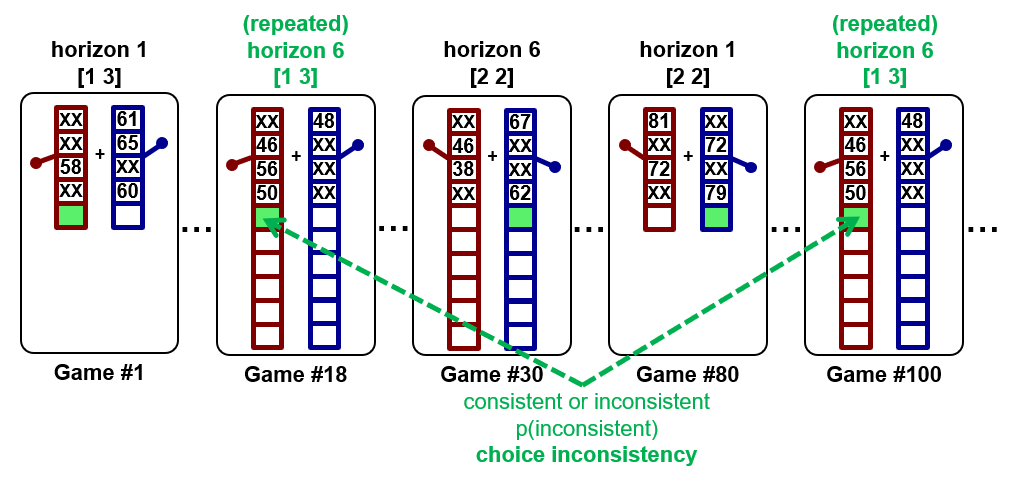
\includegraphics[width=\textwidth]{figures/task.PNG}
			\caption{A key additional manipulation here is repeated games. Each pair of repeated games with identical example trials will appear twice during the experiment. We setup the repeated games such that they are at least 5 games apart from each other. A model-free measure of choice inconsistency which reflex the underlying decision noise is defined as the proportion of inconsistent choices for repeated games.}
			\label{fig:task2}
		\end{center}
	\end{figure}
	
	Finally, the crucial additional manipulation in this task is repeated games (Figure \ref{fig:task2}). In each pair of repeated games, the four forced-choice trials were yoked, meaning that on the first free choice trial participants were faced with identical stimuli.  After the first free choice trial, the outcomes on the repeated games were not yoked and the outcomes were sampled independently from the underlying Gaussian distribution.  Not yoking the later trials made it harder for participants to detect repeated games.  In addition, the presentation of repeated games was controlled so that each repeated pair was at least five games away from each other. 
	
	\subsection*{Random exploration is dominated by internal noise}
	
	In this section we use both model-free and model-based analyses to show that both internal and external noise contribute to the behavioral variability in random exploration. Using the model-based hierarchical Bayesian analysis, we also show that the effect of internal noise is the main source of noise in random exploration.
	
	\subsubsection*{Model-free analysis}
	
	In the model-free analysis we asked whether participants' choices were  consistent or inconsistent in the two repetitions of each game.  The idea behind this measure is that purely external noise should lead to consistent choices as the external stimulus is identical both time.  Conversely, internal noise should lead to independent choices, and hence possible inconsistent choices both times. More specifically, we look at the proportion of times that a participant make inconsistent decisions in repeated game. 
	
	%used choice inconsistency in the repeated games as a measure of internal noise.  
	In addition, whether participants make consistent choices in repeated games is used as a model-free measure of internal noise, since in repeated trials, external noise should be identical on both trials. So only internal noise can differ and drive the choice inconsistency. The degree to which people make consistent choices in repeated trials can reflect the internal noise. Since choice inconsistency increases with horizon, this is a behavioral evidence that internal noise increases with horizon.
	
	\begin{figure}[H]
		\begin{center}
			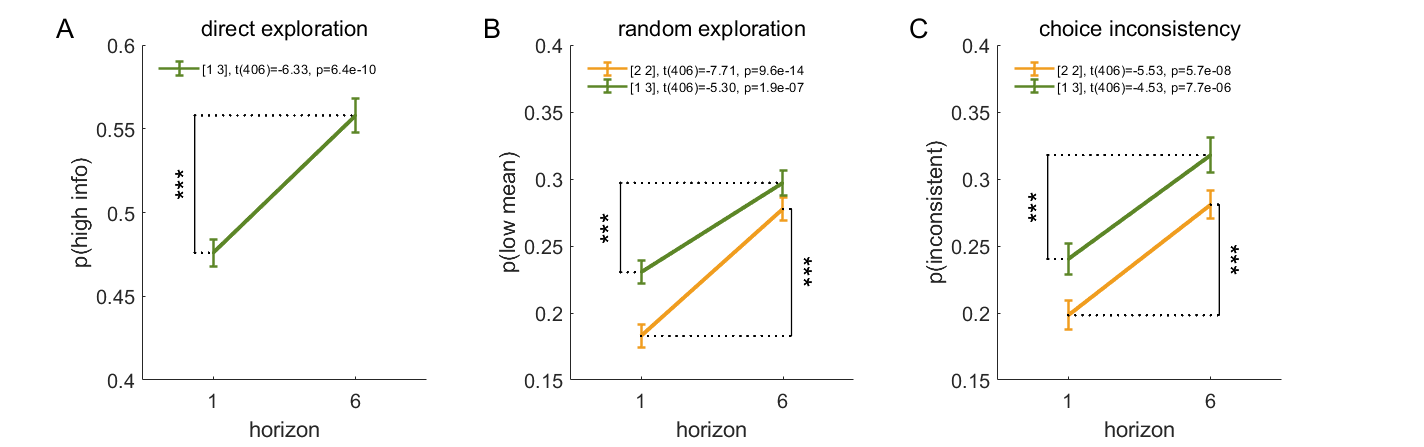
\includegraphics[width=\textwidth]{figures/Modelfree.png}
			\caption{Both direct (t(406)=-6.33, p $<$ 0.001) and random exploration (t(406) = -5.30, p $<$ 0.001 for [1 3], t(406) = -7.71, p $<$ 0.001 for [2 2]) increases with horizon.(A,B) Choice consistency in both [1 3] and [2 2] condition increases with horizon(P([1 3]) $<$ 0.001, P([2 2])$<$0.001).(C)}
			\label{fig:mf}
		\end{center}
	\end{figure}
	
	Choice inconsistency between repeated games was non-zero in both horizon conditions, suggesting that not all of the noise was stimulus driven.  In addition, choice inconsistency was higher in horizon 6 than in horizon 1 for both [1 3] and [2 2] condition (Figure \ref{fig:mf}), suggesting that at least some of the horizon dependent noise is internal.
	
	\begin{figure}[H]
		\begin{center}
			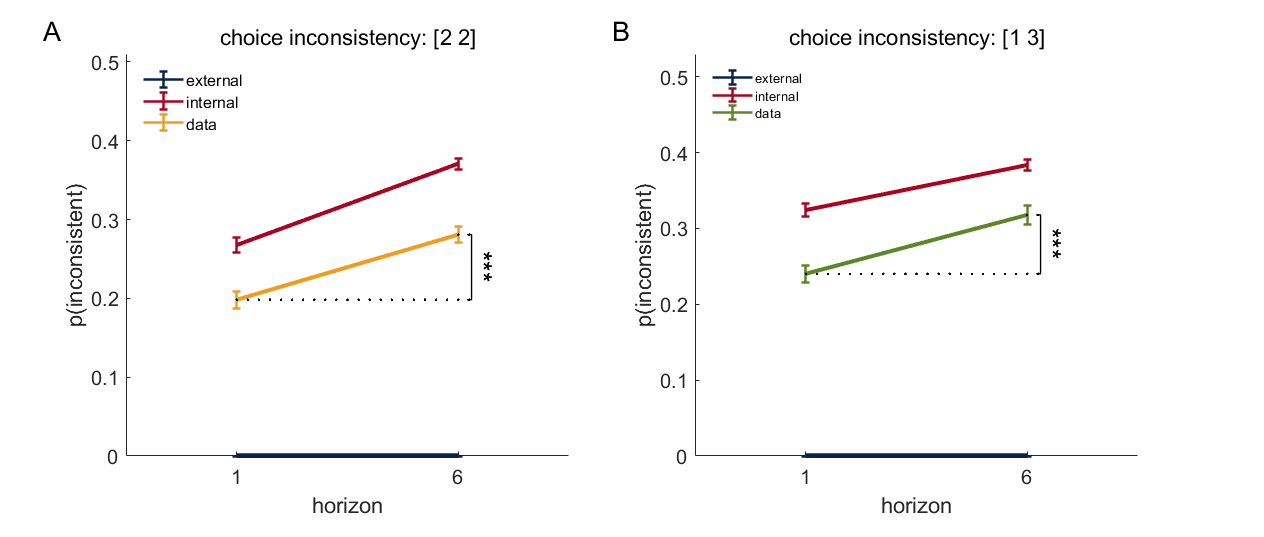
\includegraphics[width=\textwidth]{figures/modelfree_intext.png}
			\caption{For both [1 3] and [2 2] condition, there is a significant difference between people's behavior and predicted choice inconsistency assuming that only external noise exists where people should behave identically in repeated games. Also, there is a significant difference between people's behavior and predicted choice inconsistency assuming that only internal noise exists where people treat repeated games independently. }
			\label{fig:mf2}
		\end{center}
	\end{figure}
	
	To gain more quantitative insight into the data we computed predicted values of the choice inconsistency for the purely external and purely internal noise cases.  For the purely externally driven noise case, then people should make the exact same decisions each time in repeated games, which corresponds to the light blue line in Figure \ref{fig:mf2}. If noise is however purely internally driven, then there should be no stimulus-dependent noise component such that people should in principle treat repeated games independently, hence 
	\begin{equation*}
	\begin{split}
	P(\mbox{consistency}) &= P(\mbox{low mean})^2 + P(\mbox{high mean})^2\\
	&= P(\mbox{low mean})^2 + (1-P(\mbox{low mean}))^2\\ \mbox{hence},\quad P(\mbox{inconsistency}) &= 1 - P(\mbox{consistency})
	\end{split}
	\end{equation*},
	
	we can make the prediction of p(disagree) if there is only internal noise. However, people's behavior falls in between the pure external noise prediction and the pure internal noise prediction, suggesting that both external and internal noise are present in driving this choice inconsistency.
	
	Since choice inconsistency only reflects internal noise, Figure \ref{fig:mf2} suggests that internal noise increases with horizon, however we can not draw any obvious conclusions about whether external noise is horizon dependent or not.
	
	\subsubsection*{Model-based analysis}
	To more precisely quantify the size of internal and external noise in this task, we turned to model fitting.
	
	\paragraph{Overview of model}
	As with our model-free analysis, the model-based analysis focuses only on the first free-choice trial since that is the only free choice when we have control over the information bias between the two bandits. To model participants’ choices on this first free-choice trial, we assume that they make decisions by computing the difference of value $\Delta Q$ between the right and left options, choosing right when $\Delta Q > 0$ and left otherwise.  Specifically, we write
	
	
	\begin{equation}
	    \Delta Q= \Delta R+A \Delta    I+b+n_{ext}+n_{int}
	\end{equation}
	
	Where, the experimentally controlled variables are $\Delta R=R_{right}-R_{left}$, the difference between the mean of rewards shown on the forced trials, and $\Delta I$, the difference information available for playing the two options on the first free-choice trial. For simplicity, and because information is manipulated categorically in the Horizon Task, we define $\Delta I$ to be +1, -1 or 0: +1 if one reward is drawn from the right option and three are drawn from the left in the [1 3] condition, -1 if one from the left and three from the right, and in [2 2] condition, $\Delta I$ is 0). $n_{ext}$ and $n_{int}$ are external noise and internal noise respectively.
	
	The subject-and-condition-specific parameters are: the spatial bias, $b$, which determines the extent to which participants prefer the option on the right, the information bonus $A$, which controls the level of directed exploration, $n_{ext}$ denotes the external, external noise, which is identical on the repeat versions of each game, and $n_{int}$ denotes internal noise, which is uncorrelated between repeat plays. 
	
	For each pair of repeated games, the set of forced-choice trials are exactly the same, so the external noise, $n_{ext}$, should be the same while the internal noise, $n_{int}$ may be different. This is exactly how we distinguish external noise from internal noise. In symbolic terms, for repeated games i and j,  $n_{ext}^i=n_{ext}^j$  and $n_{int}^i \neq n_{int}^j$.
	
\paragraph{Model fitting}
	We used hierarchical Bayesian analysis to fit the parameters of the model (see Figure \ref{fig:model} for an graphical representation of the model in the style of CITE). In particular, we fit values of the information bonus $A$, spatial bias $B$, variance of internal noise $\sigma_{int}^2$, and variance of external noise, $\sigma_{ext}^2$ for each participant in each horizon and uncertainty condition. The mean and standard deviation of information bonus $A$ and spatial bias $B$ are sampled from a Gaussian prior and an exponential prior respectively. The variance for both type of noises were sampled from a gamma distribution, and the group-level parameter $k$ and $\lambda$ for the gamma distribution are sampled from exponential priors. 
	
	To capture the idea that external noise should be identical on repeated games, we sampled one value of the external noise, $n_{ext}$ for each pair of repeated games.  Conversely, because internal noise is expected to change between games we sampled two values of the internal noise, $n_{int}^1$ and $n_{int}^2$, i.e. one for each individual game.  
	
	The model in Figure \ref{fig:model} is fitted using the MATJAGS  and JAGS software \cite{}.
	
	\begin{table}[H]
		\small
		\begin{center}
			\begin{tabular}{|c|c|c|c|}
				\hline
				Parameter &
				Horizon dependent? &
				Uncertainty dependent? &
				Game dependent? \\
				\hline
				information bonus, $A$ &
				yes &
				n/a &
				no \\
				\hline
				spatial bias, $B$ &
				yes &
				yes &
				no \\
				\hline
				external decision noise, $\sigma_{ext}$ &
				yes & 
				yes &
				no \\
				\hline
				internal decision noise, $\sigma_{int}$ &
				yes & 
				yes &
				yes \\
				\hline
			\end{tabular}
		\end{center}
		\caption{Model parameters. }
		\label{table1}
	\end{table}%
	
	
	%Before presenting the results of the model-based analysis we begin with a brief overview of the most salient points of the model.  A full description of the model can be found in the Methods and code to implement the model can be found in the Supplementary Material.  
	
	%Conceptually, the model breaks the explore-exploit choice down into two components: a learning component, in which participants estimate the mean payoff of each option from the rewards they see, and a decision component, in which participants use this estimated payoff to guide their choice.  The learning component assumes that participants compute an estimate of the average payoff for each slot machine, $R^i_t$, using a simple delta rule update equation (based on a Kalman filter \cite{Kalman1960-uo}, see Methods):
	%\begin{equation}
	%R^i_{t+1}= R^i_t + \alpha_t^i (r_t - R^i_t)
	%\end{equation}
	%where $r_t$ is the reward on trial $t$ and $\alpha_t^i$ is the time-varying learning rate that determines the extent to which the prediction error, $(r_t - R^i_t)$, updates the estimate of the mean of bandit $i$. The learning process is described by three free parameters: the initial value of the estimated payoff, $R_0$, and two learning rates, the initial learning rate, $\alpha_1$, and the asymptotic learning rate, $\alpha_{\inf}$, which together describe the evolution of the actual learning rate, $\alpha_t$, over time. For simplicity, we assume that these parameters are independent of horizon and uncertainty condition (Table 1).
	
	%The decision component of the model assumes that participants choose between the two options (left and right) probabilistically according to 
	%\begin{equation}
	%	p(\mbox{choose right}) = \frac{1}{ 1 + \exp \left( \frac{\Delta R + A \Delta I + B}{\sigma}\right) }
	%\end{equation}
	%where $\Delta R$ ( $= R^{left}_t - R^{right}_t$ ) is the difference in expected reward between left and right options and $\Delta I$ is the difference in information between left and right options (which we define as +1 when left is more informative, -1 when right is more informative, and 0 when both options convey equal information in the [2 2] condition). The decision process is described by three free parameters: the information bonus $A$, the spatial bias $B$, and the decision noise $\sigma$.  We estimate separate values of the decision parameters for each horizon and (since the information bonus is only used in the [1 3] condition) separate values of only the bias and decision noise for each uncertainty condition. 
	
	
	
	
	
	%Overall, subject's behavior in each session (vertex vs RFPC stimulation) is described by 13 free parameters (Table \ref{table1}): three describing learning ($R_0$, $\alpha_1$ and $\alpha_{\infty}$) and 10 describing the decision process ($A$ in the two horizon conditions, $B$ and $\sigma$ in the four horizon-x-uncertainty conditions). These 13 parameters were fit to each subject in each stimulation condition using a hierarchical Bayesian approach \cite{Lee2014-yh} (see Methods).  
	
	\paragraph{Model fitting results} 
	
	Group-level estimates for the variances of internal and external noise are shown in Figure \ref{fig:modelbased}A.  While both variances are non-zero, this shows that the internal noise is much larger than external noise. This horizon-based change is probed further in Figure XXXB in which we plot the posterior distributions over the change in internal and external noise with horizon.  This clearly shows that only internal noise varies with horizon (STATS XXX\% of the samples above zero for internal noise, XXX\% of samples above zero for external noise).
	
	%LEFT EACH TYPE OF NOISE IN EACH HORIZON
	%RIGHT IS DISTRIBUTION OVER CHANGE IN NOISE WITH HORIZON
	
	%Posterior distributions over the group-level means of the external and internal noise variance are shown in Figure \ref{fig:modelbased}.  As is clear from this plot, only internal noise increases  with horizon. 
	%In both horizon 1 and horizon 6, internal noises are significantly higher than internal noises (for both horizon 1 and horizon 6, P $<$ 0.001).
	
	\begin{figure}[H]
		\begin{center}
			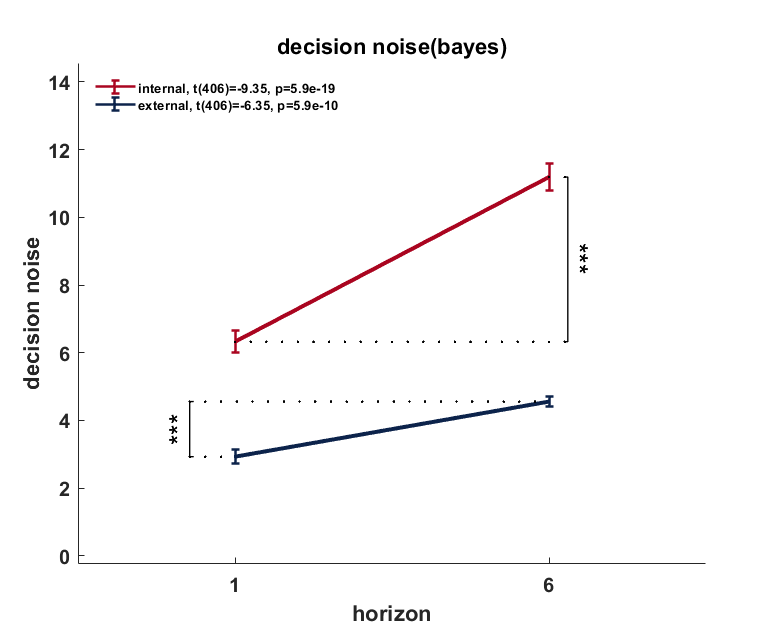
\includegraphics[width=0.5\textwidth]{figures/bayes.png}
			\caption{Both internal and external noises increase significantly with horizon.}
			\label{fig:modelbased}
		\end{center}
	\end{figure}
	
	\begin{figure}[H]
		\begin{center}
			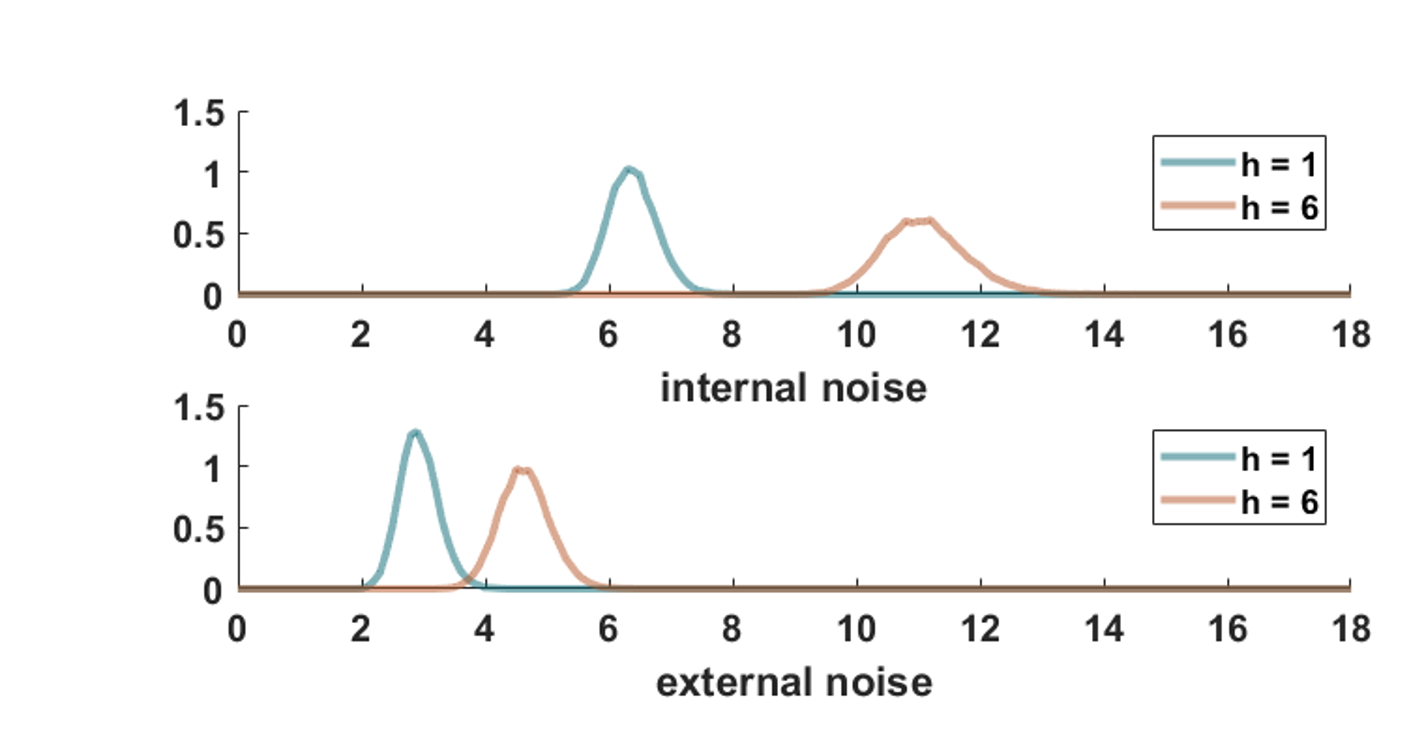
\includegraphics[width=0.5\textwidth]{figures/bayesdist.png}
			\caption{The posterior distribution of internal and external decision noise.}
			\label{fig:modelbased}
		\end{center}
	\end{figure}
	
	\begin{figure}[H]
		\begin{center}
			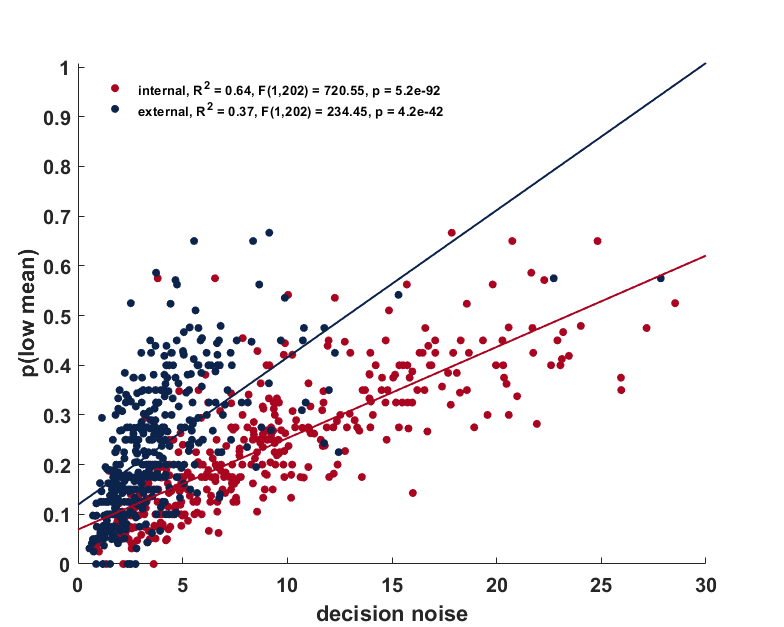
\includegraphics[width=0.5\textwidth]{figures/s1.png}
			\caption{Both internal and external noise contribute to random exploration, internal noise is dominant.}
			\label{fig:modelbased}
		\end{center}
	\end{figure}

	\section*{Discussion}
	In this paper, we investigated whether random exploration is driven by internal noise, putatively arising in the brain, or external noise, arising from the environment.  We find horizon dependent changes in both internal and external sources of noise, but that the effect of internal noise is much greater. 
	
	One limitation of this work is in the interpretation of the different noises as being internal and external. In particular, while we controlled many aspects of the stimulus across repeated games (e.g. the outcomes and the order of the forced trials), we could not perfectly control all stimuli the participant received which, for example, would vary based on where they were looking. Thus, our estimate of external noise is likely a lower bound. Likewise, our estimate of internal noise is likely an upper bound as these `missing' sources of stimulus driven noise would be interpreted as internal noise in our model. Despite this, the sheer magnitude of the difference between internal and external noise (internal noise is 2-3 times the size of external noise, Figure XXX), suggests that our interpretation may be safe as an awful lot of external noise would have to be explained by variables not relevant to the task.  
	
	
	The horizon-dependent increase in internal noise is consistent with the idea that random exploration is driven by intrinsic variability in the brain. This is in line with work in the bird song literature in which song variability during song learning has been tied to neural variability arising from specific areas of the brain.   In addition, this work is consistent with a recent report from Ebitz et al [7] in which the behavioral variability of monkeys in an `explore' state was also tied to internal rather than external sources of noise. 
	
	Whether such a noise-controlling area exists in the human brain is less well established, but one candidate theory [4] suggests that norepinephrine (NE) from the locus coeruleus may play a role in modulating internal levels of noise.  While there is some evidence that NE plays a role in explore-exploit behavior [8], this link has been questioned [9].
	
	MORE GENERALLY, OUT FINDING THAT INTERNAL DOMINATES BEHAVIORAL VARIABILITY OVER EXTERNAL NOISE, IS CONSISTENT WITH FINDINGS OF DRUGOWITSCH ET AL.  IN PARTICULAR THESE AUTHORS SHOW THAT 
	LINK IN THE Jan Drugowitsch stuff on variability.  ALEX POUGET STUFF. INTERNAL NOISE COMES FROM COMPUTATIONAL ERRORS IN COMPUTING THE CORRECT STRATEGY IN LONG  HORIZON CONDITIONS.
	
	
	THREE IDEAS
	    NOISE ADDED TO THE PROCESS
	    ATTENTION = DECREASE SIGNAL VS INCREASE NOISE
	    NOT NOISY BUT WRONG
	    PLANNING WITH FEW SAMPLES DEEP EXPLORATION
	    
	
	
	\section*{Methods}
	\subsection*{Participants}
	A total of 204 participants from the UA subject pool did the task in 4 different experiments. \\
	 017\\ 
	 49 out of 148 participants are included for analysis. 59 were excluded because of the passive condition. 59 were excluded on the basis of performance (using the same exclusion criterion as in [2]) leaving 49 for the analysis.\\
	075\\ 
	 58 out of 78 participants are included for analysis. 3 were excluded because of young age, 17 were excluded on the basis of performance (using the same exclusion criterion as in [2]) leaving 49 for the analysis.\\
	personality \\
	 65 out of 91 participants are included for analysis. 26 were excluded on the basis of performance (using the same exclusion criterion as in [2]) leaving 65 for the analysis.\\
     test-retest \\
	 33 out of 45 participants are included for analysis. 12 were excluded on the basis of performance (using the same exclusion criterion as in [2]) leaving 33 for the analysis.\\
	 
	 There are no differences of p(low mean) or p(inconsistent) across studies. No differences were found between ages, races and ethnicities.
	
	%31 healthy right-handed, adult volunteers (19 female, 12 male; ages 19-32). An initial sample size of 16 was chosen based on two studies using a very similar cTBS design that stimulated lateral FPC (Costa et. al. 2011; 2013) and this was augmented to 31 on the basis of feedback from reviewers. 5 participants (5 female, 0 male) were excluded from the analysis due to chance-level performance in both experimental sessions. One (female) participant failed to return for the second (vertex stimulation condition) session and is excluded from the model-free analyses but not the model-based analyses as that can handle missing data more gracefully. Thus our final data set consisted of 25 participants (13 female, 12 male, ages 19-32) with complete data and one participant (female, aged 20) with data from the RFPC session only.
	
	%All participants were informed about potential risks connected to TMS and signed a written consent. The study was approved by University of Social Sciences and Humanities ethics committee.
	
	%\subsection*{Procedure}
	%There were two experimental TMS sessions and a preceding MRI session.  On the first session T1 structural images were acquired using a 3T Siemens TRIO scanner. The scanning session lasted up to 10 minutes. Before the first two sessions, participants filled in standard safety questionnaires regarding MRI scanning and TMS. During the experimental sessions, prior to the stimulation participants went through 16 training games to get accustomed to the task. Afterwards, resting motor thresholds were obtained and the stimulation took place. Participants began the main task immediately after stimulation. The two experimental sessions were performed with an intersession interval of at least 5 days. The order of stimulation conditions was counterbalanced across subjects. All sessions took place at Nencki Institute of Experimental Biology in Warsaw.
	
	%\subsection*{Limitations}
	
	%Defining stimulation target by peak coordinates based on findings from previous studies did not allow to account for individual differences in either brain anatomy or the impact of TMS on brain networks \cite{Gratton2013-wz}. However, a study by Volman and colleagues \cite{Volman2011-fz} that used the same theta-burst protocol on the left frontopolar cortex has shown bilateral inhibitory effects on blood perfusion in the frontal pole. This suggests that both right and left parts of the frontopolar cortex might have been inhibited in our experiment, which is consistent with imaging results indicating bilateral involvement of the frontal pole in exploratory decisions.
	
	\subsection*{Task}
	The task was a modified version of the Horizon Task \cite{}. As in the original paper, the distributions of payoffs tied to bandits were independent between games and drawn from a Gaussian distribution with variable means and fixed standard deviation of 8 points. Participants were informed that in every game one of the bandits always has a higher mean reward than the other. Differences between the mean payouts of the two slot machines were set to either 4, 8, 12 or 20. One of the means was always equal to either 40 or 60 and the second was set accordingly. The order of games was randomized. Mean sizes and order of presentation were counterbalanced. The number of games participants play depends on how well they perform, the better they perform, the sooner the task will end. On average, participants played 128 games and the whole task lasted between 39 and 50 minutes (mean 43.4 minutes). 
	
	\begin{figure}[H]
		\begin{center}
			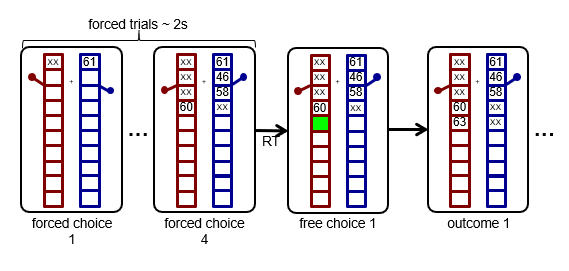
\includegraphics[width=\textwidth]{figures/taskfig1.PNG}
			\caption{Timeline of a game}
			\label{fig:modelbased}
		\end{center}
	\end{figure}
	
	Each game consisted of 5 or 10 choices. Every game started with a fixation cross, then a bar of boxes will show up indicating the horizon for that game. For the first 4 games - the instructed games, we highlight the box on one of the bandits to instruct the participant to choose that option, they have to press the corresponding key to reveal the outcome. From the $5^{th}$ trial, boxes on both bandits will be highlighted and they are free to make their own decision. There was no time limit for decisions. During free choices they could press either the left arrow key or right arrow key to indicate their choice of left or right bandit. The score feedback was presented for 500ms. The task was programmed using Psychtoolbox in MATLAB. \cite{}.
	
	
	
	
	%Finally, the random seeds were not perfectly controlled between subjects.  The first 16 subjects ran the task with identical random seeds and thus all 16 saw the same sequence of forced-choice trials in both vertex and RFPC sessions. For the remaining subjects the random seed was unique for each subject and each session, thus these subjects had unique a series of forced-choice trials for each session.  Despite this limitation we saw no evidence of different behavior across the two groups.
	
	\subsection*{Data and code}
	%Behavioral data as well as Matlab code to recreate the main figures from this paper can be found on the Dataverse website at https://dataverse.harvard.edu/dataset.xhtml?persistentId=doi:10.7910/DVN/CZT6EE.
	
	
	\subsection*{Model-based analysis}
	We modeled behavior on the first free choice of the Horizon Task using a version of the logistic choice model in \cite{} that was modified to differentiate internal and external noises. In particular, we assume that in repeated games, external noise remains the same whereas internal noise can change. 
	
	%\subsubsection*{Decision component}
	%Once the payoffs of each option, $R^i_t$, have been estimated from the outcomes of the forced-choice trials, the model makes a decision using a simple logistic choice rule:
	%\begin{equation}
	%	p(\mbox{choose right}) = \frac{1}{ 1 + \exp \left( \frac{\Delta R + A \Delta I + B}{\sigma}\right) }
	%\end{equation}
	%where $\Delta R$ ( $= R^{left}_t - R^{right}_t$ ) is the difference in expected reward between left and right options and $\Delta I$ is the difference in information between left and right options (which we define as +1 when left is more informative, -1 when right is more informative, and 0 when both options convey equal information in the [2 2] condition). The three free parameters of the decision process are: the information bonus, $A$, the spatial bias, $B$, and the decision noise $\sigma$.  We assume that these three decision parameters can take on different values in the different horizon and uncertainty conditions (with the proviso that $A$ is undefined in the [2 2] information condition since $\Delta I = 0$). Thus the decision component of the model has 10 free parameters ($A$ in the two horizon conditions, and $B$ and $\sigma$ in the 4 horizon x uncertainty conditions).  Directed exploration is then quantified as the change in information bonus with horizon, while random exploration is quantified as the change in decision noise with horizon.
	
	\subsection*{Model Fitting}
	\subsubsection*{Hierarchical Bayesian Model}
	Each subject's behavior is described by 4 free parameters. These parameters are: the information bonus, $A$, in both horizon conditions, the spatial bias, $B$, in the four horizon x uncertainty conditions, and external decision noise, $n_{int}$, and internal decision noise, $n_{ext}$ in the four horizon x uncertainty conditions (Table \ref{tab:pars2}, Figure \ref{fig:model}). 
	
	Each of the free parameters is fit to the behavior of each subject using a hierarchical Bayesian approach \cite{}.  In this approach to model fitting, each parameter for each subject is assumed to be sampled from a group-level prior distribution whose parameters, the so-called `hyperparameters', are estimated using a Markov Chain Monte Carlo (MCMC) sampling procedure. The hyper-parameters themselves are assumed to be sampled from `hyperprior' distributions whose parameters are defined such that these hyperpriors are broad.  
	
	The particular priors and hyperpriors for each parameter are shown in Table \ref{tab:pars2}. For example, we assume that the information bonus, $A^{is}$, for each information condition x horizon condition $i$, is sampled from a Gaussian prior with mean $\mu^{A}_{i}$ and standard deviation $\sigma_{i}^A$. These prior parameters are sampled in turn from  their respective hyperpriors: $\mu_{i}^{A}$, from a Gaussian distribution with mean 0 and standard deviation 10, $\sigma_{i}^A$ from an Exponential distribution with parameters 0.1.
	
	\begin{table}[H]
		\small
		\begin{tabular}{|c|c|c|c|}
			\hline
			Parameter & Prior & Hyperparameters & Hyperpriors \\
			information bonus, $A_{is}$ 
			& $A_{is} \sim $  Gaussian($\mu_i^{A}$, $\sigma_i^{A}$) 
			& $\theta_{i}^{A} = (\mu_i^{A}, \sigma_i^{A}) $
			& \specialcell{
				$\mu_i^{A} \sim $ Gaussian( 0, 100 ) \\ 
				$\sigma_i^{A} \sim $ Exponential(0.1)}		\\
			\hline
			spatial bias, $B_{is}$ 
			& $B_{is} \sim $  Gaussian($\mu_i^{B}$, $\sigma_i^{B}$) 
			& $\theta_{i}^{B} = (\mu_i^{B}, \sigma_i^{B}) $
			& \specialcell{
				$\mu_i^{B} \sim $ Gaussian( 0, 100 ) \\ 
				$\sigma_i^{B} \sim $ Exponential(0.1)}		\\
			\hline
			external decision noise, $\epsilon_{isg}$ 
			& $\epsilon_{isg} \sim $  Gaussian(0, $\sigma_{is}^{ext}$) 
			& $\theta_{i}^{ext} = (k_i^{ext}, \lambda_i^{ext}) $
			& \specialcell{
				$k_i^{ext} \sim $ Gaussian(0.1) \\ 
				$\lambda_i^{ext} \sim $ Exponential(10)}		\\
			\hline
			internal decision noise, $\sigma_{isgr}$ 
			& $\sigma_{isg} \sim $  Gaussian(0, $\sigma_{is}^{int}$) 
			& $\theta_{i}^{int} = (k_i^{int}, \lambda_i^{int}) $
			& \specialcell{
				$k_i^{int} \sim $ Gaussian(0.1) \\ 
				$\lambda_i^{int} \sim $ Exponential(10)}		\\
			\hline
		\end{tabular}
		\caption{Model parameters, priors, hyperparameters and hyperpriors.}
		\label{tab:pars2}	
	\end{table}
	
	\subsubsection*{Model fitting using MCMC}
	The model was fit to the data using Markov Chain Monte Carlo approach implemented in the JAGS package \cite{} via the MATJAGS interface (psiexp.ss.uci.edu/research/programs\_data/jags/).  This package approximates the posterior distribution over model parameters by generating samples from this posterior distribution given the observed behavioral data.  
	
	In particular we used 4 independent Markov chains to generate 40000 samples from the posterior distribution over parameters (10000 samples per chain).  Each chain had a burn in period of 1000 samples, which were discarded to reduce the effects of initial conditions, and posterior samples were acquired at a thin rate of 1.  Convergence of the Markov chains was confirmed post hoc by eye. Code and data to replicate our analysis and reproduce our Figures is provided as part of the Supplementary Materials.
	
	\begin{figure}[H]
		\begin{center}
			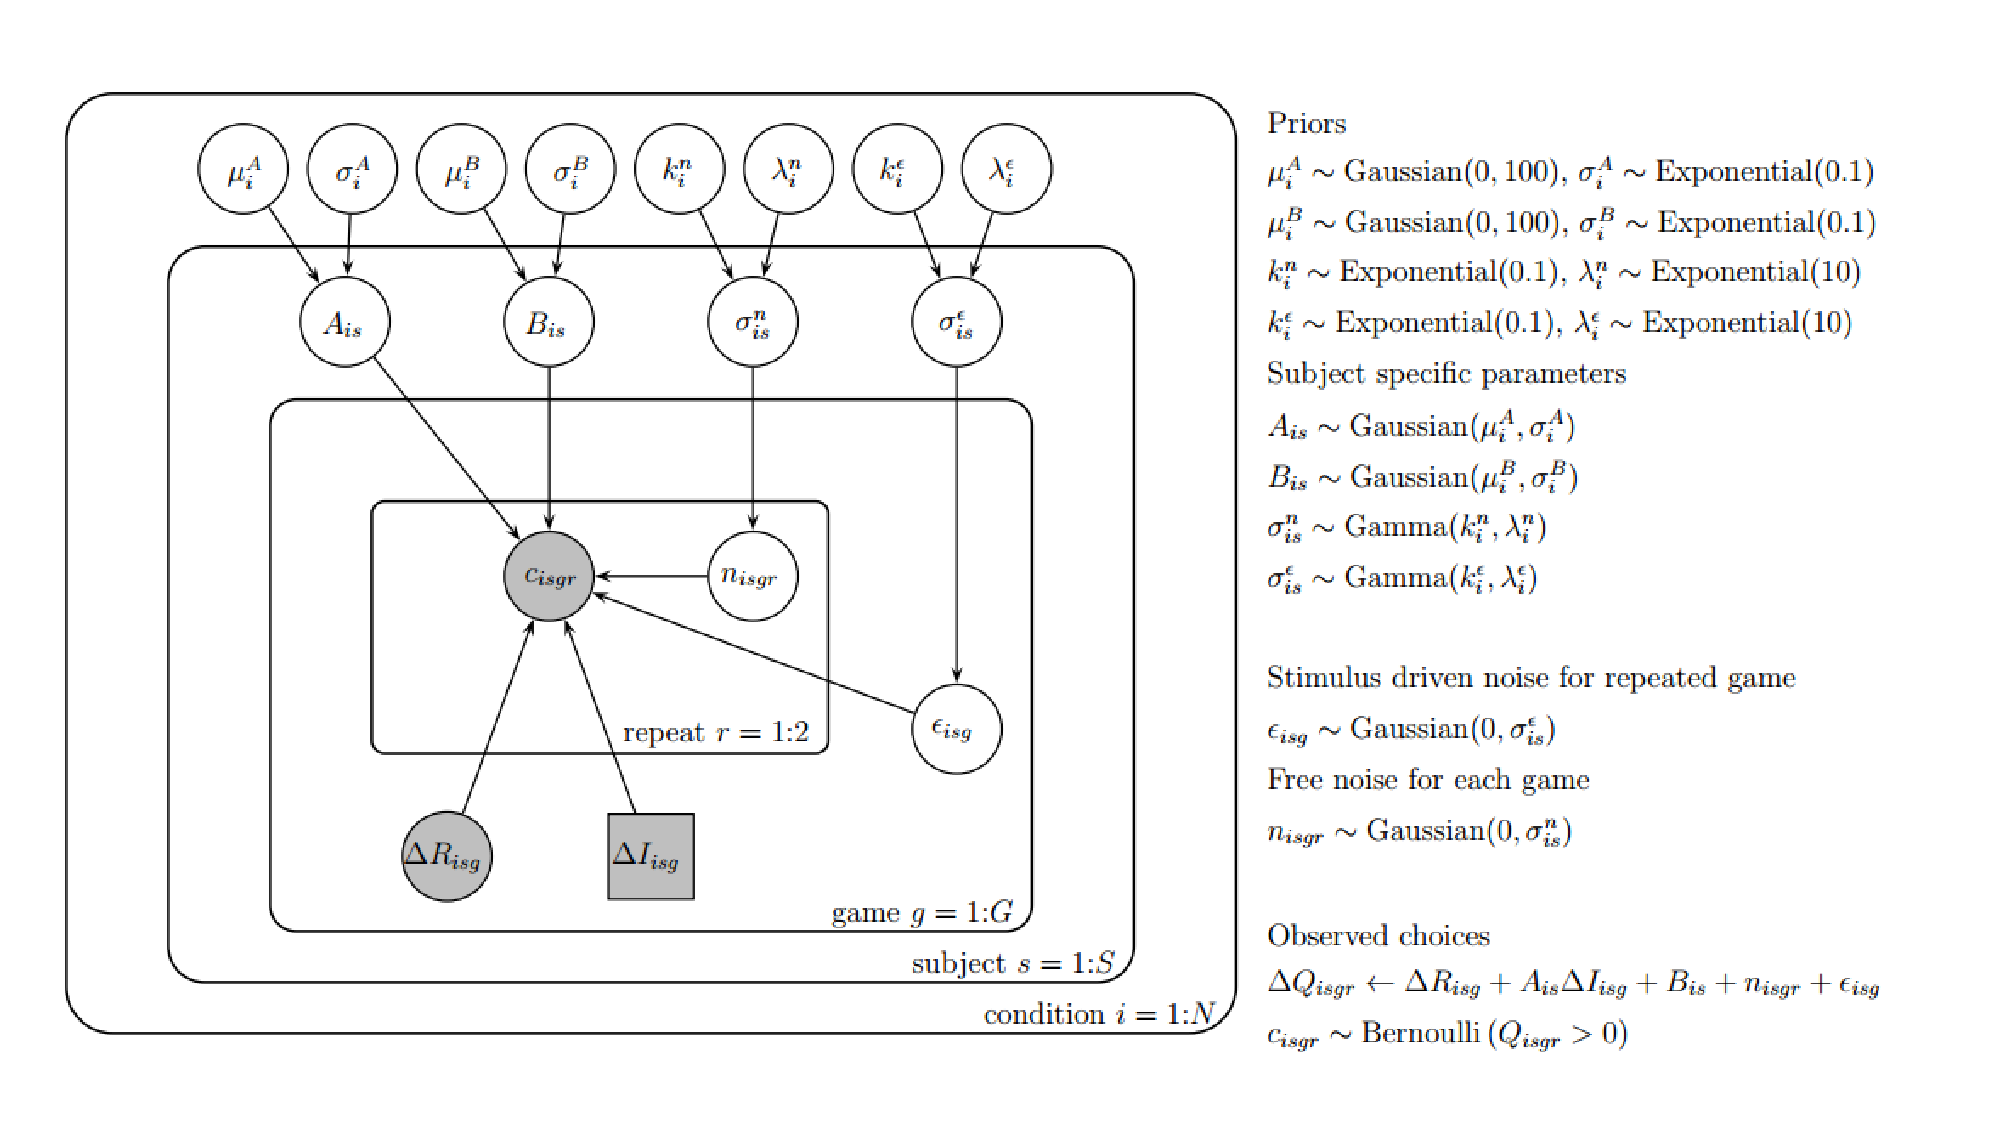
\includegraphics[width=\textwidth]{figures/Figure3.pdf}
			\caption{Hierarchical Bayesian model}
			\label{fig:model}
		\end{center}
	\end{figure}
	%References
	%Plummer, M. (2003, March). JAGS: A program for analysis of Bayesian graphical models using Gibbs sampling. In Proceedings of the 3rd international workshop on distributed statistical computing (Vol. 124, p. 125).
	%Rescorla, R. A., & Wagner, A. R. (1972). A theory of Pavlovian conditioning: Variations in the effectiveness of reinforcement and nonreinforcement. Classical conditioning II: Current research and theory, 2, 64-99.
	
	
	
	\bibliographystyle{apalike}
	\bibliography{references}
	
	
\end{document}
